\begin{figure}[t]
    \centering
    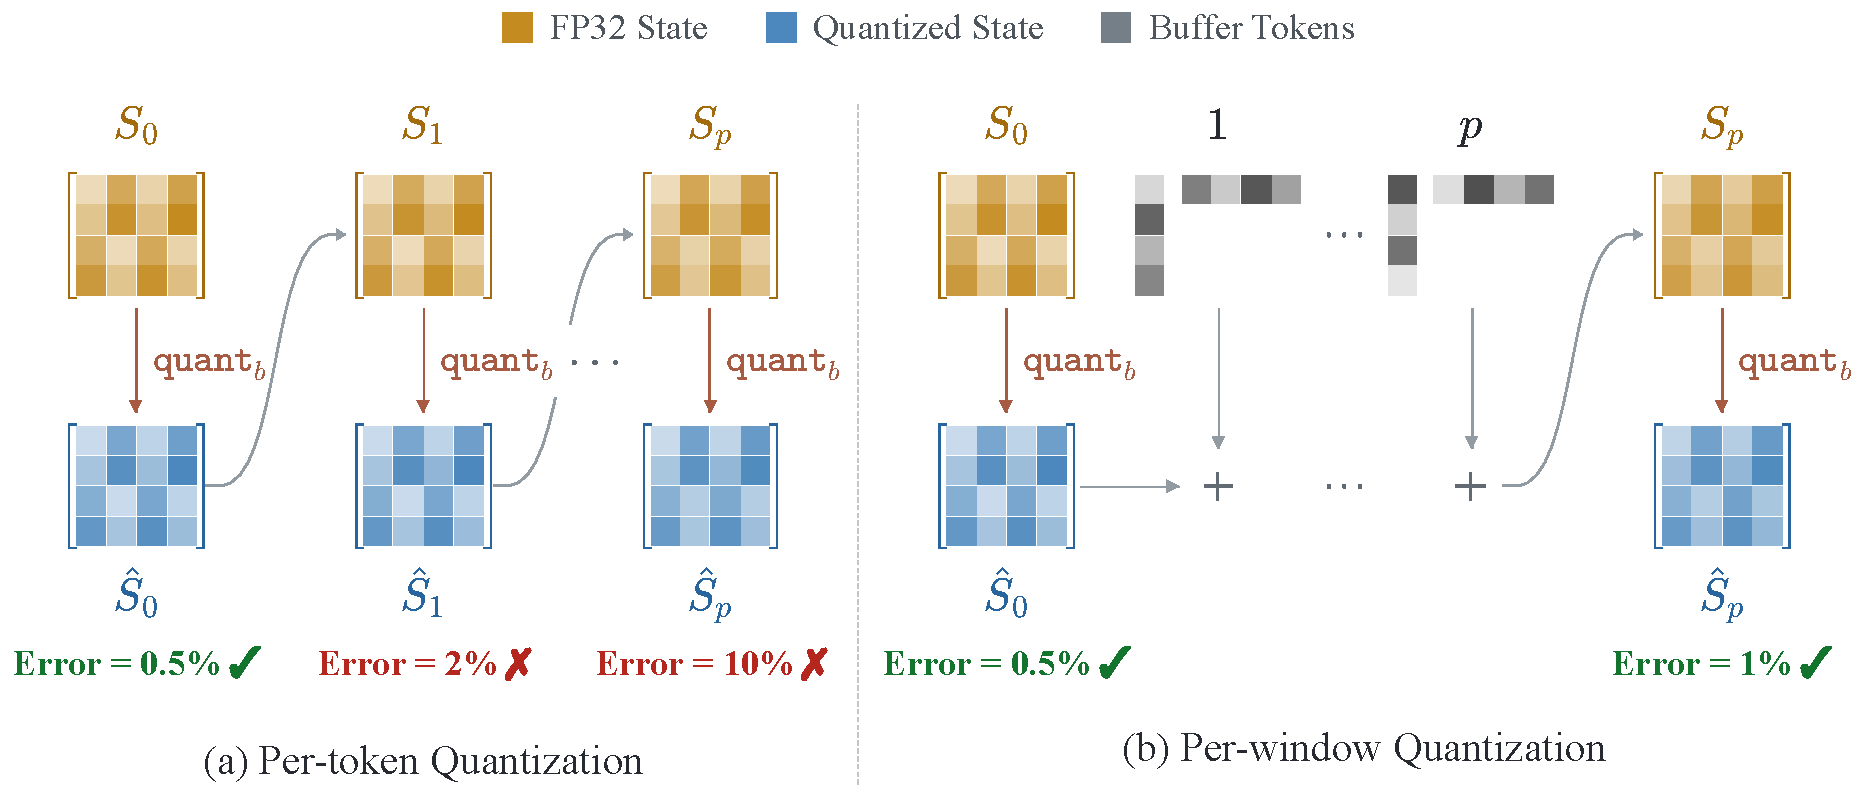
\includegraphics[width=0.9\linewidth]{figures/per-window-quantization-paper.pdf}
    \caption{Per-token versus per-window quantization. Per-token quantization re-quantizes the full state after every update. Per-window quantization holds the quantized boundary state $\hat S_0$ fixed, buffers the $p$ updates of the window in higher precision, and reconstructs the state from them; the full state is quantized only once per window, into $\hat S_p$.}
    \label{fig:per-window}
    \vspace{-1.5em}
\end{figure}
